\documentclass[11pt,a4paper]{article}
\usepackage[utf8]{inputenc}
\usepackage[margin=2.5cm]{geometry}
\usepackage{amsmath}
\usepackage{amsfonts}
\usepackage{amssymb}
\usepackage{booktabs}
\usepackage{graphicx}
\usepackage{float}
\usepackage{hyperref}
\usepackage{natbib}
\usepackage{tikz}
\usetikzlibrary{shapes,arrows}

\title{Hospital Readmission Prediction Using Clinical Notes:\\A Natural Language Processing Approach}
\author{Ichim Ștefan}
\date{\today}

\begin{document}

\maketitle

\section{Problem Statement}

Hospital readmissions within 30 days of discharge represent a critical healthcare challenge with significant implications for patient outcomes and healthcare costs. This project addresses the binary classification task of predicting hospital readmissions using unstructured clinical notes through Natural Language Processing techniques.

The classification problem is formally defined as:
\begin{equation}
f: X \rightarrow \{0, 1\}
\end{equation}
where $X$ represents processed clinical notes from hospital admission, and the output indicates readmission status within 30 days (0 = no readmission, 1 = readmission).

\section{Proposed Solution}

This study implements and compares three distinct transformer-based approaches for hospital readmission prediction using clinical notes from the MIMIC-III dataset:

\textbf{Clinical BERT Baseline:} The first approach establishes a baseline using the Bio\_ClinicalBERT model with standard fine-tuning procedures. This approach applies basic text preprocessing and utilizes a standard classification head to predict 30-day readmission risk from clinical notes.

\textbf{BioBERT with Named Entity Recognition:} The second approach leverages BioBERT enhanced with Named Entity Recognition preprocessing. This method first extracts structured clinical entities (symptoms, medications, diagnoses) from the unstructured text, then uses these extracted features alongside the original text for classification, providing richer semantic representation.

\textbf{Clinical BERT Enhanced:} The third approach optimizes the Clinical BERT architecture through multi-layer classifier enhancement and gradient accumulation techniques. This method implements an expanded classifier head (768→2048→768→1) and uses gradient accumulation to achieve larger effective batch sizes, improving training stability and model performance.

Each approach leverages domain-specific pre-trained models while exploring different strategies for clinical text processing and model optimization to determine the most effective methodology for readmission prediction.

\section{Theoretical Aspects}

\subsection{Formal Description of Methods}

The transformer-based approaches utilize multi-head attention mechanisms:
\begin{equation}
\text{Attention}(Q, K, V) = \text{softmax}\left(\frac{QK^T}{\sqrt{d_k}}\right)V
\end{equation}

Final classification probability is computed as:
\begin{equation}
P(y=1|x) = \sigma(W_c \cdot h_{[CLS]} + b_c)
\end{equation}
where $h_{[CLS]}$ is the classification token representation, $W_c$ and $b_c$ are learned parameters, and $\sigma$ is the sigmoid function.

For handling long clinical notes exceeding BERT's 512-token limit, subsequence aggregation is applied:
\begin{equation}
P_{final} = \frac{P_{max} + P_{mean} \cdot \frac{n}{c}}{1 + \frac{n}{c}}
\end{equation}
where $P_{max}$ is maximum probability among subsequences, $P_{mean}$ is mean probability, $n$ is number of subsequences, and $c = 2.0$.

\subsection{Dataset Used in Application}

The MIMIC-III database serves as the primary data source, containing de-identified health data from approximately 40,000 patients in critical care units at Beth Israel Deaconess Medical Center (2001-2012).

\begin{table}[H]
\centering
\caption{Dataset Characteristics}
\begin{tabular}{@{}lr@{}}
\toprule
\textbf{Characteristic} & \textbf{Value} \\
\midrule
Total Admissions & 36,438 \\
Training Set & 25,506 (70\%) \\
Validation Set & 5,466 (15\%) \\
Test Set & 5,466 (15\%) \\
Readmission Rate & 5.98\% \\
Readmission Window & 30 days \\
Note Categories & Discharge Summary \\
\bottomrule
\end{tabular}
\end{table}

\subsection{Application}

The application framework consists of two main phases: data preprocessing and model training/evaluation. The preprocessing pipeline transforms raw clinical text through cleaning, medical artifact removal, temporal filtering, age filtering, and note aggregation. This process converts raw clinical text $T_{raw}$ into processed text $T_{processed}$ through:
\begin{equation}
T_{processed} = \text{Aggregate}(\text{Filter}(\text{Clean}(T_{raw})))
\end{equation}

The overall workflow follows a systematic approach where preprocessed clinical notes are fed into the three different model architectures, each trained using 5-fold cross-validation, and evaluated using AUROC metrics. The general application flow is illustrated below:

\begin{figure}[H]
\centering
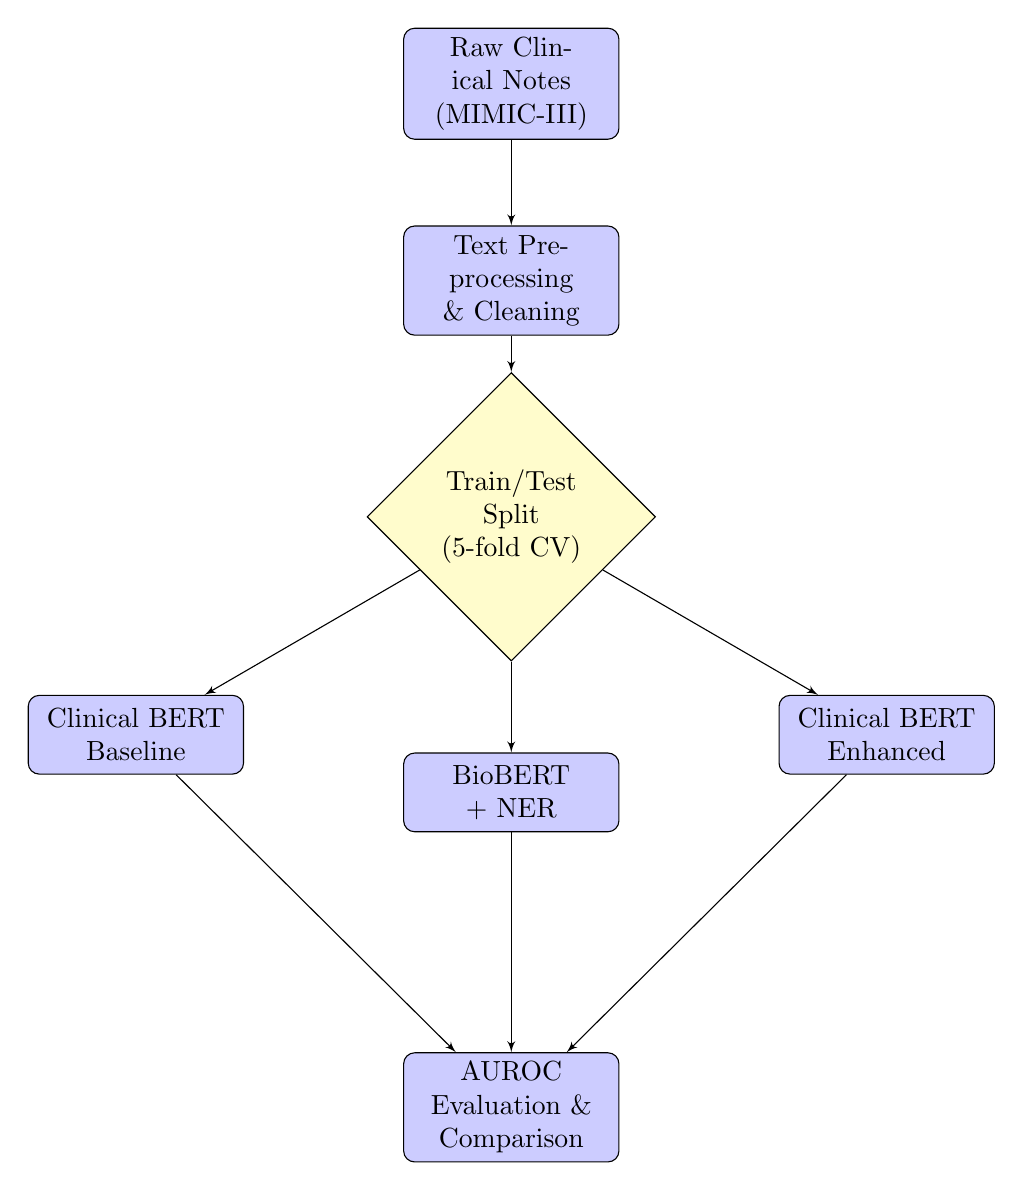
\begin{tikzpicture}[node distance=2.5cm, auto]
\tikzstyle{block} = [rectangle, draw, fill=blue!20, text width=2.5cm, text centered, rounded corners, minimum height=1cm]
\tikzstyle{decision} = [diamond, draw, fill=yellow!20, text width=2cm, text centered, minimum height=1cm]
\tikzstyle{line} = [draw, -latex']

\node [block] (raw) {Raw Clinical Notes (MIMIC-III)};
\node [block, below of=raw] (preprocess) {Text Preprocessing \& Cleaning};
\node [decision, below of=preprocess, yshift=-0.5cm] (split) {Train/Test Split (5-fold CV)};
\node [block, below left of=split, xshift=-3cm, yshift=-1cm] (bert1) {Clinical BERT Baseline};
\node [block, below of=split, yshift=-1cm] (bert2) {BioBERT + NER};
\node [block, below right of=split, xshift=3cm, yshift=-1cm] (bert3) {Clinical BERT Enhanced};
\node [block, below of=bert2, yshift=-1.5cm] (eval) {AUROC Evaluation \& Comparison};

\path [line] (raw) -- (preprocess);
\path [line] (preprocess) -- (split);
\path [line] (split) -- (bert1);
\path [line] (split) -- (bert2);
\path [line] (split) -- (bert3);
\path [line] (bert1) -- (eval);
\path [line] (bert2) -- (eval);
\path [line] (bert3) -- (eval);
\end{tikzpicture}
\caption{General Application Workflow for Hospital Readmission Prediction}
\end{figure}

The framework enables systematic comparison of the three approaches under identical experimental conditions, ensuring fair evaluation of their relative performance in predicting 30-day hospital readmissions from clinical text data.

\section{Implementation Details}

\begin{table}[H]
\centering
\caption{Implementation Overview for Three Approaches}
\begin{tabular}{@{}llll@{}}
\toprule
\textbf{Component} & \textbf{Clinical BERT} & \textbf{BioBERT + NER} & \textbf{Clinical BERT Enhanced} \\
\midrule
Base Model & Bio\_ClinicalBERT & BioBERT & Bio\_ClinicalBERT \\
Preprocessing & Text cleaning & NER + Text cleaning & Advanced text cleaning \\
Architecture & Standard classifier & Standard classifier & Multi-layer classifier \\
Max Sequence Length & 512 tokens & 512 tokens & 512 tokens \\
Batch Size & 8 & 8 & 8 \\
Learning Rate & 2e-5 & 2e-5 & 2e-5 \\
Training Epochs & 3 & 3 & 3 \\
Special Features & Basic fine-tuning & Named entity extraction & Gradient accumulation \\
\bottomrule
\end{tabular}
\end{table}

\begin{table}[H]
\centering
\caption{Model Architecture Details}
\begin{tabular}{@{}ll@{}}
\toprule
\textbf{Component} & \textbf{Configuration} \\
\midrule
Base Model & emilyalsentzer/Bio\_ClinicalBERT \\
Hidden Size & 768 \\
Classifier Layers & 768 → 2048 → 768 → 1 \\
Activation Functions & ReLU \\
Loss Function & BCEWithLogitsLoss \\
Optimizer & AdamW \\
Gradient Clipping & 1.0 \\
Cross-Validation & 5-fold stratified \\
\bottomrule
\end{tabular}
\end{table}

Key preprocessing functions include robust age calculation using nanosecond precision and comprehensive text cleaning with regex patterns for clinical text normalization. The text cleaning function removes PHI markers, normalizes line breaks and medical degree abbreviations, and standardizes whitespace.

\section{Experiments and Results}

All experiments were conducted using 5-fold stratified cross-validation to ensure robust evaluation across different data splits while maintaining the original class distribution. Model performance was assessed using the Area Under the Receiver Operating Characteristic Curve (AUROC), which measures the model's ability to distinguish between patients who will be readmitted and those who will not across all classification thresholds.

The AUROC metric ranges from 0 to 1, where 0.5 indicates random performance and 1.0 represents perfect classification. This metric is particularly suitable for clinical prediction tasks as it provides a threshold-independent measure of discriminative ability, crucial for identifying patients at risk of readmission regardless of the specific decision threshold chosen for clinical implementation.

\begin{table}[H]
\centering
\caption{Performance Comparison Across All Approaches}
\begin{tabular}{@{}lr@{}}
\toprule
\textbf{Approach} & \textbf{AUROC} \\
\midrule
Clinical BERT (Baseline) & 0.5729 \\
BioBERT with NER & 0.6485 \\
Clinical BERT (Enhanced) & \textbf{0.6682} \\
\bottomrule
\end{tabular}
\end{table}

\begin{table}[H]
\centering
\caption{Detailed Cross-Validation Results for Best Approach (Clinical BERT Improved)}
\begin{tabular}{@{}lrrrr@{}}
\toprule
\textbf{Fold} & \textbf{AUROC} & \textbf{Val Loss} \\
\midrule
1 & 0.6714 & 0.2173 \\
2 & 0.6748 & 0.2175 \\
3 & 0.6903 & 0.2155 \\
4 & 0.6599 & 0.2182 \\
5 & 0.6447 & 0.2210 \\
\midrule
\textbf{Mean} & \textbf{0.6682} & \textbf{0.2179} \\
\textbf{Std} & \textbf{0.0172} & \textbf{0.0020} \\
\bottomrule
\end{tabular}
\end{table}

The Clinical BERT Enhanced approach achieved the best performance with an average AUROC of 66.82\%, representing a 16.6\% relative improvement over the baseline Clinical BERT (57.29\%) and a 3.0\% improvement over BioBERT with NER (64.85\%). The model demonstrated consistent performance across folds with low standard deviation (1.72\% for AUROC) and stable training dynamics with monotonic loss decrease.

The three approaches demonstrate distinct advantages: the baseline Clinical BERT provides a foundation for clinical text understanding, BioBERT with NER incorporates structured entity recognition to enhance feature extraction, and the enhanced Clinical BERT optimizes the training process through improved architecture and gradient accumulation techniques.

The study contributes a systematic comparison of transformer-based approaches for clinical readmission prediction, demonstrating the effectiveness of architectural enhancements and training optimizations. The enhanced Clinical BERT approach provides a robust framework for clinical text analysis with improved discriminative performance. Future work should focus on addressing class imbalance through advanced techniques and exploring ensemble methods combining the strengths of different approaches.

\end{document}
